\section{Filtro LDR}
\subsection{Enunciado}

\subsection*{Filtro \textit{LDR}}
  Programar el filtro \textit{LDR} en lenguaje C y en
  ASM haciendo uso de las instrucciones \textbf{SSE}.

\vspace*{0.3cm} \noindent
\textbf{Experimento 1}

  Analizar cuales son las diferencias de performace entre las versiones de C y ASM. 
  Realizar gráficos que representen estas diferencias.
  
\subsection{An\'alisis previo}
\'Este filtro recorre todos los elementos de la im\'agen fuente, copia un marco de 2 filas y 2 columnas y lo pega en la im\'agen fuente. Para los elementos internos, 
suma todos los elementos en un cuadrado de 4x4 pixeles, con el elemento actual en el medio (para I[i][j], el cuadrado va desde I[i-2][j-2] hasta I[i+2][j+2]).
A \'esta suma que se realiza para cada pixel (con todos los colores, no por separado) se la divide por 75*255*255 y luego se lo multiplica por alfa (valor de entrada) 
y src (en su color correspondiente), para finalmente multiplicar por el valor original.

La dificultad consiste en recorrer eficientemente el cuadrado de 4x4 para hacer la sumatoria, ya que las filas no son datos contiguos en memoria.

\subsection{Implementaci\'on en C}
En C podemos ver y recorrer la submatriz de 4x4 con facilidad. Por eso, luego de usar 2 for para recorrer cada elemento de la matriz se utilizan otros dos for para 
recorrer la submatriz, sumar y guardar los elementos en variables auxiliares y luego hacer las cuentas correspondientes con cada color del pixel.
La \'unica consideraci\'on en el codigo es que, si estamos en el marco de 2 filas - 2 columnas, los pixeles se copian directamente sin procesar.


\subsection{Implementaci\'on en assembler}
La implementaci\'on en assembler varia muy poco conseptualmente. Primero verificamos que podemos aplicar la f\'ormula al estar 2 filas y 2 colulmnas dentro de la im\'agen.
\begin{codesnippet}
\begin{verbatim}
				CMP R10, 1 		;VEO SI ESTOY EN LAS PRIMERAS 2 FILAS
				JBE .copioFila
				; SI NO:
				MOV R12, RCX 
				SUB R12, R10 	;VEO SI ESTOY EN LAS ULTIMAS 2 FILAS
				CMP R12, 2
				JBE .copioFila
				; SI NO:
				CMP R11, 1 		;VEO SI ESTOY EN LAS PRIMERAS 2 COLUMNAS
				JA .else
\end{verbatim}
\end{codesnippet}


\subsection{Resultado de los experimentos}

\vspace*{0.3cm} \noindent
\textbf{Experimento 1}

\begin{figure}
  \begin{center}
	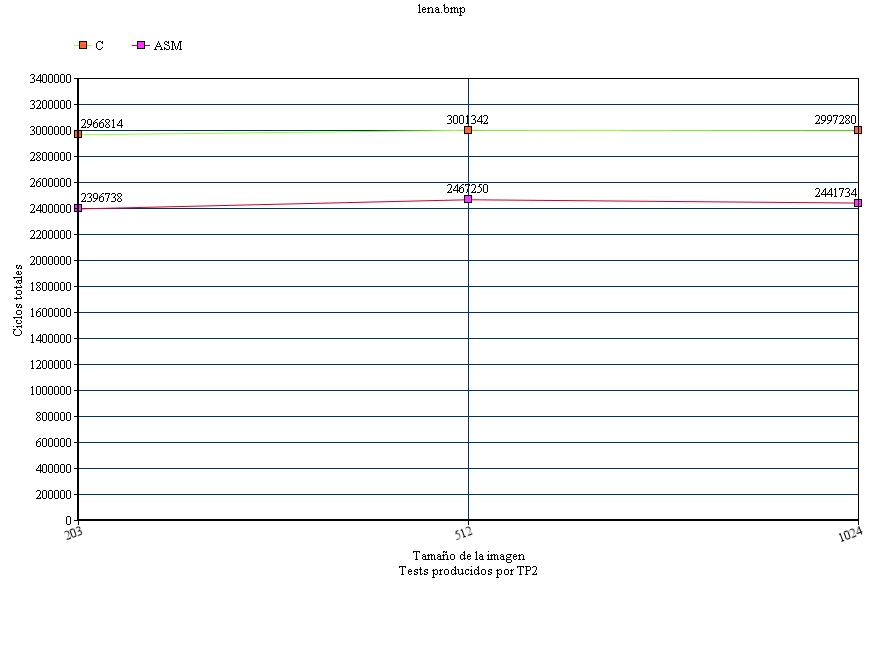
\includegraphics[scale=0.66]{imagenes/ldr-lena.jpg}
	\caption{Lena}
	\label{Lena}
  \end{center}
\end{figure}

\begin{figure}
  \begin{center}
	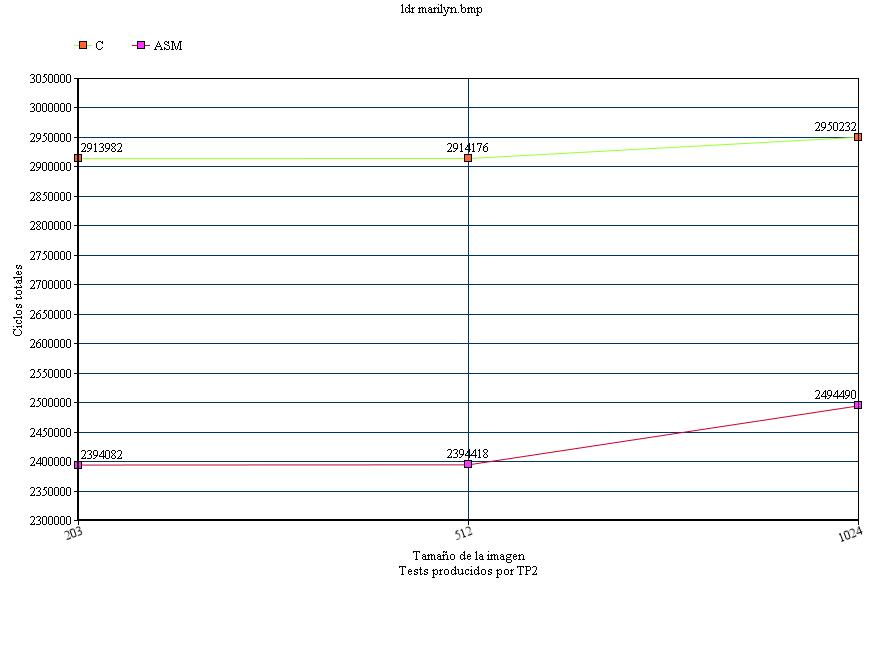
\includegraphics[scale=0.66]{imagenes/ldr-marilyn.jpg}
	\caption{Marilyn}
	\label{Marilyn}
  \end{center}
\end{figure}

Realizamos los tests armando un ciclo de 100000 ejecuciones del mismo c\'odigo con las mismas entradas, y a su vez ejecutamos estos tests 5 veces para cada entrada. \'Esto nos 
permiti\'o hacer promedios y descartar tests que daban muy lejos del valor medio.

Como muestran los gr\'aficos presentados, hay claras diferencias de velocidad (medida en cantidad de ciclos) entre uno y otro lenguaje. Tambi\'en notamos que no hay una gran 
variaci\'on de velocidad entre los distintos tamaños de las im\'agenes, as\'i como a veces las variaciones no son las esperadas. En este sentido, realizamos varias ejecuciones 
del TP2 con exactamente los mismos par\'ametros y vimos que variaban sin un patr\'on. Pensamos que si mejoraba con las sucesivas iteraciones podr\'ia ser 
producto de la acci\'on de la cache, pero como no fue as\'i vemos que tiene que ver con qu\'e tan ocupado est\'a el cpu. \'Esto no pudo ser confirmado ya que todos 
los tests se corrieron sin que ningun otro programa visible a nosotros est\'e corriendo.
\begin{figure}
  \begin{center}
	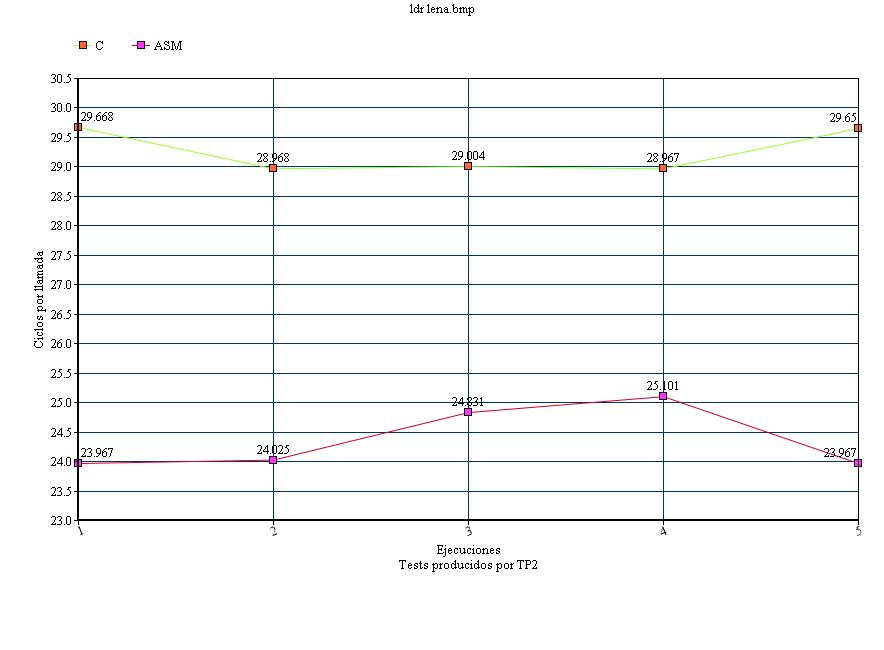
\includegraphics[scale=0.66]{imagenes/ldr-lena-203.jpg}
	\caption{lena-203x203}
	\label{lena-203x203}
  \end{center}
\end{figure}
